\section{Introduction}

\acused{atm}
For most people, interacting with touch screens provides an intuitive way of interacting with various everyday devices and appliances, from coffee machines to \acp{atm}.
This ease and intuitiveness of touch screens is one of the reasons for the prevalence of touch screens nowadays.
However, for one group of users, using touch screens without help proves to be completely impossible: the heavily visually impaired or blind people.
For general purpose devices, such as smartphones and personal computers, a variety of screen readers and helpers exist, that allow blind people to use these devices.
Examples include Google TalkBack for Android \cite{talkback} (Google Inc., Mountain View, USA), Apple VoiceOver for iOS \cite{voiceover} (Apple Inc. Cupertino, USA), and the Windows Accessibility Service for Microsoft Windows \cite{windowsaccessibility} (Microsoft Corporation, Redmond, USA). 
But as touch screens provide  no tactile feedback and most embedded, special purpose devices (such as coffee machines) do not implement alternative ways for \ac{io}, the usage of these devices becomes seemingly impossible without eyesight or without relying on the help of other people, which poses an obstacle to the everyday life and diminishes the independence of blind people.

Some research and development was done in the area of using wearables and computer vision to aid visually impaired people with various tasks.
\textcite{googleglass} propose a system to help blind or visually impaired people with basic navigation and recognition tasks using Google Glass (Google Inc., Mountain View, USA).
However, it is unclear whether their system can detect touch screens and an interaction mechanism to use touch screens was not intended.
A different, yet similar to our idea, proposal was given by \textcite{holofacility}: They use the Microsoft HoloLens (Microsoft Corporation, Redmond, USA) to supply additional information on devices, mainly intended to be used at trade fairs, where space for information material is constrained.
Although their system \enquote{HoloFacility} is not meant as an assistive technology for the visually impaired, it shares some traits with our system.

There are a number of different proposals which revolve around the usage of smart glasses to aid visually impaired people with various tasks, including some vague patents about using smart glasses as assistive devices for blind people \autocite{smartglasses, smartglasses2, smartglasses3}, but also more sophisticated system, such as the one proposed by \textcite{bai2017smart}.
It was meant to be used as an electronic travel aid for visually impaired people and could \enquote{effectively improve the user's travelling experience in complicated indoor environments} in a user study.
A patent hold by Logitech Europe SA \autocite{logitech} proposes a system for blind usage of touch interfaces.
However, their system relies on the device manufacturer implementing the system, hence it is not device-independent and not suitable for the current situation of embedded touch screens on a manifold of different devices from different manufacturers.
There are patents and devices for reading normally printed letters, some seemingly ancient \cite{ring}, some more recent \cite{ring2}.

To our knowledge, no device or system as proposed by us exists or is being developed at this time.
To be specific, no system exists that 
\begin{itemize}
	\item
		is device independent.
		Our system does not rely on any changes or cooperation by device manufacturers.
		The only requirements for a device to be used with our system is the attaching of markers next to the touch screen and the device being present in our database (see \autoref{subsec:markers}).
		Both requirements can be fulfilled by the users themselves.
	\item
		soley relies on speech and gesture \ac{io}.
		Our system uses these modes of \ac{io} as natural ways of interacting with our users, allowing us to build an intuitive \ac{ui} for using touch screen devices without eyesight.
\end{itemize}



%\begin{itemize}
	%\item
		%Blind people face challenges in everyday life
	%\item
		%Especially touchscreens are unusable for blind people
	%\item
		%What is done to help blind people use electronics? (literature review, simple past, six references)
		%\begin{itemize}
			%\item
				%Screen readers
			%\item
				%Braille keyboards
			%\item
				%Voice control
		%\end{itemize}
	%\item
		%No device-independent --  thus not relying on implementation and help by the touch-system's manufacturer -- system available to help visually impaired people use touchscreens.
	%\item
		%BlindAR is set to improve 
%\end{itemize}

\begin{comment}
The introduction describes the problem you solved and why it is important. You start with a general problem definition and subsequently a more detailed description of the problem you faced. Then, you provide existing solutions to this problem or related problems and their solution. Make sure the reader understands the differences! You HAVE to use references in this section to provide an idea what has already been done in this research area. Mainly, you cite journal articles 
%\cite{JournalArticle},
conference proceedings 
%\cite{ProceedingsArticle}
%, books \cite{Book}
and web links. 
%\cite{Weblink}. 
Having defined the body of knowledge you introduce how you are going to solve the problem. You finish with a crystal clear purpose of your project or contribution to the problem.

The literature review is written in simple past. The rest of the introduction is generally present tense. You can also use present tense for giving insight in what will be shown in the article. A rule of thumb are six references of other solutions or related projects, solutions and systems.  
\end{comment}



%Methods
\section{Methods}
In the following, we will present the different parts of our system, used algorithms and third-party libraries.


\subsection{Platform and Development Environment}
\label{subsec:sucks}
As  hardware platform we decided to use the Microsoft HoloLens as it is hands-free and does not obstruct the users from their normal tasks.
It offers information about the spatial surroundings of the user via so called \enquote{Spatial Mapping} (see \Cref{subsec:spatial}) and an easy to use speech \ac{io} system via Microsoft's Cortana (see \Cref{subsec:ui}).

We started developing with Unity (Unity Technologies, San Francisco, USA), as advised by the hardware manufacturer Microsoft, which is supposed to provide an  easy start into augmented reality development.
However, we could not get needed libraries like OpenCV to work when developing with Unity, which made us switch to developing directly with DirectX and Microsoft Visual Studio 2017.



\begin{comment}
	\begin{itemize}
		\item
			Used HoloLens (Microsoft Corporation, Redmond, Washington, USA) as hardware platform
		\item
			Started developing with Unity (Unity Technologies, San Francisco, USA), as advised by hardware manufacturer Microsoft
		\item
			Spent first few weeks with getting to know the hardware platform, Unity and the developing process
		\item
			Had trouble finding a version working for every team member
		\item
			Could not get OpenCV to work when using Unity
		\item
			Switched to developing using only Visual Studio and DirectX
		\item
			Huge part of ecosystem broke away, as Microsoft's documentation for developing apps for the HoloLens using DirectX is very sparse and we can't rely on a lot of libraries/implementations
	\end{itemize}
\end{comment}

\subsection{Marker Detection}
\label{subsec:markers}
To begin a successful interaction with any touchscreen, obviously the system first has to detect if a touchscreen is present.
This is not a trivial problem.
Touchscreens are hard to detect as reflections may occur, lighting and brightness conditions may vary and screen content is notoriously non-static.

%\begin{figure}[thpb]
%\centering
%
\includegraphics[width=0.99\columnwidth]{markers.png}
%\caption{Possible markers for the HoloLensARToolKit \cite{artoolkit}, similar markers are used with ArUco \cite{aruco}}
%\label{fig:markers}
%\end{figure}

Thus, we decided to use a marker-based approach to touchscreen detection, where users are required to put markers next to touchscreens.
This places a small burden of initially placing the markers on users---which we believe is acceptable---but drastically reduces the complexity of touchscreen detection.

Because we faced technical problems with using either the HoloLensARToolKit \cite{artoolkit}  or the OpenCV marker detection module ArUco \cite{aruco}, we decided to implement our own marker detection pipeline.
\acused{api}
We used the webcam stream, readily available via the HoloLens \ac{api}.
First, we applied grayscaling, then regular and Otsu thresholding, and finally a difference edge detector, which leaves us with \autoref{fig:finalmarker}.
To further process the marker, the warped and twisted marker image from \autoref{fig:markerdetection} had to be transformed into a quadratic form.
Then a $5\times5$ grid could be overlaid, creating a grid representation of the marker image, allowing the encoded data to be read from the marker.
The data was represented as an unsigned integer -- a unique ID, identifying the exact device, e.g.\ coffee machine X by manufacturer Y.

\begin{figure}[thpb]
	\centering
	\begin{subfigure}[t]{0.45\columnwidth}
		\centering
		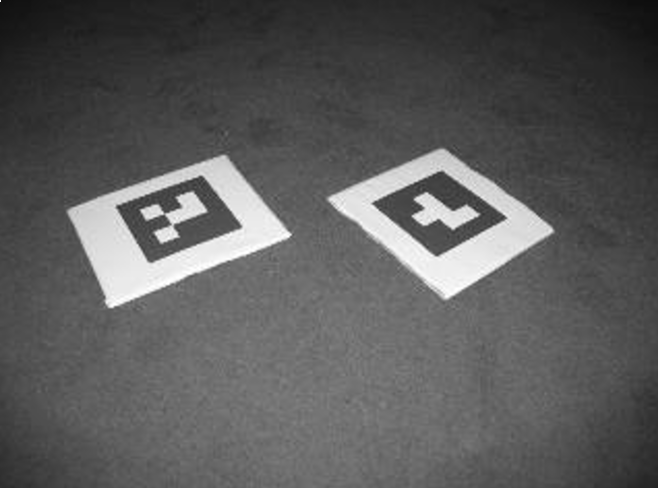
\includegraphics[width=\columnwidth]{gray.png}
		\caption{Sample image after grayscaling}
		\label{fig:gray}
	\end{subfigure}
	\begin{subfigure}[t]{0.45\columnwidth}
		\centering
		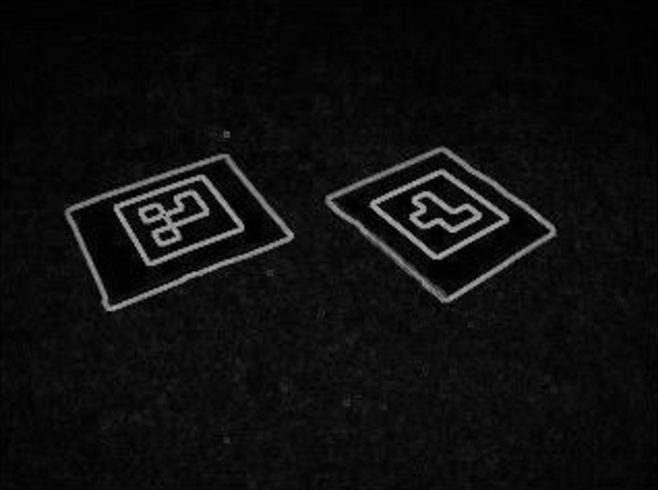
\includegraphics[width=\columnwidth]{thresh.png}
		\caption{Image after applying regular thresholding}
		\label{fig:thresh}
	\end{subfigure}
	\begin{subfigure}[b]{0.45\columnwidth}
		\centering
		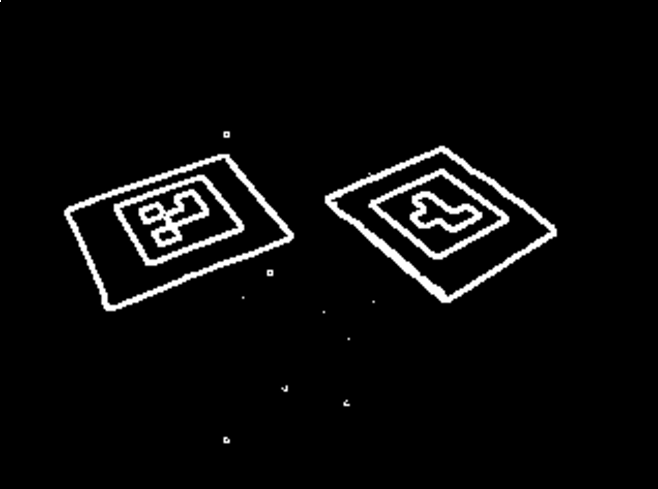
\includegraphics[width=\columnwidth]{otsu.png}
		\caption{Image after applying Otsu thresholding}
		\label{fig:otsu}
	\end{subfigure}
	\begin{subfigure}[b]{0.45\columnwidth}
		\centering
		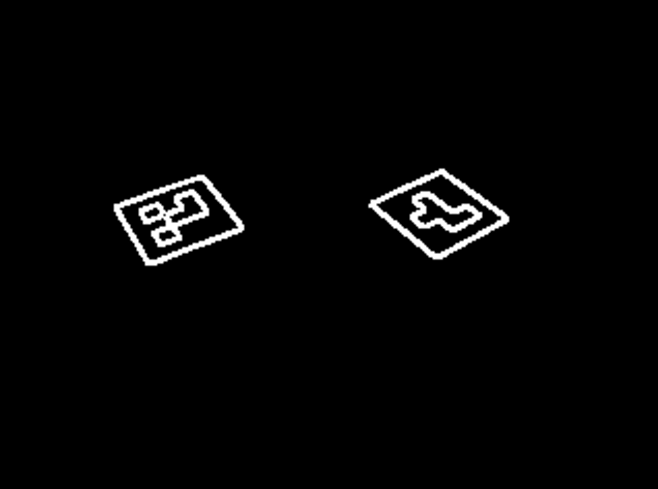
\includegraphics[width=\columnwidth]{edge.png}
		\caption{Image after applying a difference edge detector} \label{fig:finalmarker}
	\end{subfigure}
	\caption{Visualisation of marker detection pipeline steps}
	\label{fig:markerdetection}
\end{figure}

The complete data on devices then could be loaded, either from local storage (as in  our case a \texttt{.json} file) or from a remote database\footnote{which also could be community maintained/crowdsourced}.
Data includes the screen size and the position and size of each (touch-)button with an appropriate string describing the button (e.g.\ \enquote*{a}, \enquote*{b}, \dots{} for a virtual keyboard or \enquote{Espresso}, \enquote{Cappuccino},~\dots{} for buttons on a coffee machine).
This button layout is saved for each possible screen that can be shown by the touch screen.
At this point  the system knows about the existence of a touch screen in its vicinity and the possible screen contents that can be shown.
To determine which of many possible screens is shown at one time and create a virtual, blind-friendly representation, \ac{ocr} is used.

\subsection{Optical Character Recognition}
\label{subsec:ocr}
\ac{ocr} is needed to  to determine which screen content is actually shown and to determine if button presses were successful.
For this task, we used the Microsoft \ac{ocr} Library for Windows Runtime.
Besides 19 other languages, it is able to excellently recognize German and English, which were the main languages we focused on.

The text returned from the \ac{ocr} then was compared with the text of buttons stored in the screen layouts. 
Using minimal edit distance  -- to account for possible recognition errors -- as a comparison metric, we were able to determine the current screen layout.
For optimal, error free interaction with the touch screen device, the system needs to know the exact position and orientation of the touch screen in the 3D space around the user.
This is accomplished using the \emph{Spatial Mapping} provided by the HoloLens.

\subsection{Spatial Mapping}
\label{subsec:spatial}
According to the \textcite{spatialmapping}, spatial mapping provides \enquote{a detailed representation of real-world surfaces in the environment around the HoloLens}.
For this task, the HoloLens is equipped with two cameras in the center of the forehead, which use Time-of-Flight to estimate the distance to objects and surfaces around the user. 
The spatial mapping \ac{api} returns \emph{spatial surfaces}, represented as a triangle mesh.
A visualisation of such a mesh can be seen in \Cref{fig:spatialmesh}.

\begin{figure}[thpb]
	\centering
	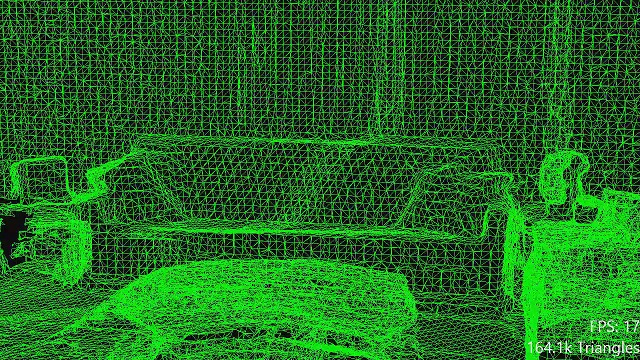
\includegraphics[width=\columnwidth]{spatialmapping.jpg}
	\caption{Visualisation of a spatial mesh \cite{spatialmapping}}
	\label{fig:spatialmesh}
\end{figure}

Using raycasting, we were able to find the position of the markers on the spatial surface.
Combined with the information from the touch screen database (size of screen, position of buttons, \dots) this allowed us to construct a \enquote{virtual touchscreen} consisting of virtual cubes and cuboids, accurately aligned with the corresponding real world touch screen buttons, \emph{in front} of the actual touch screen, which the user then can interact with (see \Cref{subsec:ui}).


\subsection{Finger Tracking}
\label{subsec:finger}
For both modes  of interaction, an accurate position of the user's finger is needed.
The HoloLens \ac{api} could give us the position of the center of the user's  back of the hand.
Thus, we had to find a different means of tracking the user's finger.

The Leap Motion (Leap Motion Inc., San Francisco, USA) seemed to be promising and delivered formidable results with regards to accuracy and ease of use.
However, it had the big drawback of needing a permanent cable connection to a full-fletched PC which was too much of a burden on the usability of the system to continue using it.

Our first own approach was to just use the HoloLens \ac{api} provided hand position and add a static offset to it.
This proved accurate enough for testing but not for real world deployments:
What if a user has really small hands?

Again our fallback solution was OpenCV.
We wrapped the user's fingertip with a colored tap (e.g.\ red, green or blue), then filtered the webcam stream for that color, mapped that dot into 3D space and thus had a reliable and accurate finger position.
One possible usability improvement would be to filter the webcam stream for the user's skin color and use this for finger tracking.
This already has been done by \textcite{fingertips}, but we did not reimplement his solution.


\subsection{Speech Input and Output and User Interface}
\label{subsec:ui}
\label{subsec:voiceio}
For speech \ac{io}, we decided to use Microsoft's Cortana as it was readily available via it's easy to use \ac{api}.
If a supported touch screen device was detected in the user's vicinity, its presence was indicated to the user, who subsequently could choose between two modes of interaction: the \emph{verbose} mode and the \emph{normal} mode.

\subsubsection{The verbose mode}
The user announced to the system, that they wished to use the touch screen via a voice command.
Then the system read out all the information shown on the touch screen to the user.
Via voice command the user selected one button they wished to press.
The system guided the user's finger to the selected button via \enquote{spatial beeping}.

The HoloLens offers a spatial sound \ac{api}, allowing developers to seemingly play sounds as they were coming from specified 3D coordinates around the user.
Combined with a beeping sound that varies in beeping frequency proportional to the finger's distance to the selected button, effectively allowing the user to quickly move their finger to the button's position.

\subsubsection{The normal mode}
The normal mode was meant for users that  are already familiar with some devices around them.
When a touch screen's presence was indicated to the users, they could chose to not engage the system via a voice command but instead just hover their finger over the touch screen.
If the finger collided with a button of the virtual touchscreen -- consisting of cuboids floating in front of the real touch screen -- that buttons text was read out.
This allowed for much quicker interactions.

\begin{comment}
This section includes everything the reader needs to understand your system and results. Things you just used only have to be mentioned and cited. For data recording, we used the mobile system developed by Kugler et al.
%\cite{ProceedingsArticle}.
Make sure to describe your contribution as short and precise as possible and as detailed as needed to reimplement it. You have to include a description of data, hardware, math, algorithms, system structure and evaluation methods and everything that was important to solve the defined problem. Make sure to order the methods so that the reader can follow your description. First things first! Make sure to structure the methods in a proper way. Use a dry description and try not to teach the reader. \\
The methods part is written in simple past, even if you created a live system that can still do things. It is only important what the system did on the data you presented. Only describe the best and final version of the system. The reader is not interested what you did wrong in developing the final system. Things that did not work don't have to be mentioned.

	\subsection{Structure}
	A rule of thumb is that you describe one fact in each paragraph. That means, if you go to the next aspect, you start with a new paragraph. Try to maintain a logical structure throughout the paper where paragraphs build upon each other.\\
	A good way to structure the paper are subsections. You can also use enumerations to structure the paper. Use an unordered list if the items don't have a structure.
	\begin{itemize}
		\item Apple
		\item Peach
		\item Melon
		\item Grape
	\end{itemize}
	Use an ordered list if there is a hierarchical structure in the list.
	\begin{enumerate}
		\item Erlangen
		\item Bavaria
		\item Germany
		\item Europe
	\end{enumerate}
	You should always have more than one subsection. Otherwise the structure does not make sense.

	\subsection{Figures, equations and tables}
	Add figures and cite the figures at the end of a sentence (Fig.~\ref{einstein}). Good figures make a paper a lot better. Don't use figures if they are of bad quality or not exactly what you want to show with it. Latex puts figures where they fit best regarding the document structure. Often, figures are not at the same place as they are defined in the source code. Don't worry too much about that. Often, they are place on top of a page but the desired (not defined) positioning can be specified in the brackets after begin\{figure\}. Make sure the figure is readable when printed in black and white. This means that the lines in a plot have to be of different shape (dotted, dashed,\dots) and the coloring has to be adapted if used. Print the paper in black and white if unsure.\\
	Add important equations that a relevant for understanding your system and cite them (Eq.~\ref{einstein}). Every variable has to be explained. The variable $f$ denotes the force, $m$ the mass and $c$ a constant. Make sure to reference the equation or provide an explanation. When writing about value make sure to insert a safe blank between value and unit like 9.81~g or 67~\% to avoid a line break between value and unit. The safe blank is also needed when referencing figures.

	\begin{equation}
		f = m \times c^2
		\label{einstein}
	\end{equation}

	\subsection{Proper use of language}
	Make sure to use proper English in your papers. Get the paper reviewed by another person to avoid stupid typos and check the language for common mistakes. If the paper is important, try to find a native speaker for review. Some common language related problems:
	\begin{itemize}
		\item Make sure to use lower case for nouns.
		\item There are no strict rules for punctuation in English and, in some cases, the rules are different to German rules. One common problem is the use of a comma in a relative clause. There is no comma after ``that'' and ``which'' if it is a restrictive relative clause like ``The book which I read is well written.''. There is a comma if it is a non-restrictive relative clause like ``That book, which incidentally I just finished reading, is well written.''. A rule of thumb is that you use a comma if the relative sentence is not needed to make it a proper sentence.
		\item Use short sentence in paratactic form. This is easier to read. Long sentences are hard to understand. You don't write poems that are supposed to be of nice language.
		\item You can alternate between active and passive. Contrary to German, the use of active is also elegant. When talking about yourself you should write ``the author'' or ``we''. 
		\item Do not abbreviate terms like ``do not'', ``cannot'' or ``it is''.
		\item Find scientific synonyms for colloquial language. You can start colloquial and then transform into scientific language afterwards. If you are unsure how to start you can use a phrasebank 
			%	\cite{Phrasebank}
			to copy nice formulations.
		\item If you are not sure if you found the right word in a dictionary use a single language dictionary like %\cite{Weblink}.
		\item Numbers: write words when referring to numerals below ten, referring to fractions, referring to approximate numbers and at the beginning of a sentence. Use figures when referring to sets of numbers, numbers including decimal points and when referring to pages. Make sure to use a decimal point instead of a comma as in German. 
		\item	Get yourself inspired from the literature. Use nice formulations from other papers. Never copy words but copy style.  
	\end{itemize} 
	It is very important to be consistently in wording and punctuation. Call the same things with the same name even if you think that it is boring. Use the same punctuation rule throughout the complete paper. 

\subsection{Template and length}
You should always avoid to change the template. It was created for a good reason. If your manuscript is too long you should change the content and not the template. Concentrate on the purpose of your project and get rid of side aspects. Use references and keep work of others short. You HAVE to learn to describe your work in a given length. A rule of thumb is a partitioning of 15 \% (Introduction), 40 \% (Methods), 10 \% (Results), 25 \% (Discussion) and 10 \% (Summary and outlook).

\subsection{Source code and devices}
Normally, you don't present source code. The reader is more interested in a flow chart to understand how your algorithm works.  Describe the most important steps of algorithms in detail and briefly describe other parts. Always provide a version when referring to other software packages or libraries. 
If you talk devices like smart phones or treadmills provide the manufacturer and the companies headwater details like (Google Inc., Mountain View, USA). 
\end{comment}

%Results
\section{Results}
We tried to validate our system by doing a small user study, recruiting the subjects from the \ac{bbsb}, the Bavarian society for the visually impaired.
We contacted them and sent out a short survey, asking them about their use of assistive technologies and impairments they face in everyday life.

You describe the pure results in this section. Performance measures, reference system and experimental setup have to be explained in the methods part. Don't provide an interpretation of the results in this section, just talk about the results. Don't provide reasons why your system didn't work in this or that condition. Just mention that this was the case. Quantitative results are most striking and you might want to sum them up in a table (Tab.~\ref{result_table}). If you have a lot of different results, pick the best and most important ones. Focus on the purpose of your system! You can use the same structure as in the methods section if appropriate.\\
The result section is written in simple past. Even if you have a live system, you describe the results as achieved in the evaluation. 

%\begin{table}[!t]
	%\caption{The caption in tables has to be self explaining like in figures (see Fig.). Make sure to explain all abbreviations that you use in the caption.}
	%\begin{center}
		%\begin{tabular}{c|cccccccccc}
			%& \ S1 \ &\ S2 \ &\ S3 \ & \ S4 \ & \ S5 \ & \ S6 \ & \ S7 \ & \ S8 \ & \ S9 \ & \ S10\\
			%\hline
			%RULE&0.5&0.7&0.3&0.7&0.8&0.2&0.3&0.5&0.7&0.9\\
			%EPIC&0.1&0.1&0.1&0.1&0.1&0.1&0.1&0.1&0.1&0.1\\
		%\end{tabular}
		%\label{result_table}
	%\end{center}
%\end{table}

%Discussion
\section{Discussion}
Begin with a short problem specific summary. Discuss every aspect from the result section and give an interpretation of the results. You can use the same structure as in the results. Why is the algorithm so good/bad? What are limitations or assumptions? What was remarkable in the project and can be seen in the data. Make sure to cite the literature when comparing to existing systems or algorithms. Always mention pros and cons! Discuss global strength and weakness and concentrate on major aspects.\\
The discussion is mainly written in simple past. You can use present tense when talking about facts that you are absolutely sure about. If you are very self confident, you can deduce facts from your findings but often conditional formulations are more polite. Sometimes it is better to combine the discussion with an outlook so you might want to use future as well. 

%Discussion
\section{Summary and outlook}
Sum up the most important project findings and mention what the next steps, improvements, enhancements could be. The outlook can consist of ideas that will be hard to realize. Don't just think about tomorrow, think about the next ten years. You can finish with advertising your work and point out the most important finding or development again.\\
The summary part is written in simple past. The outlook is written in present tense or future.
